% ===================================================================
% SKILL: NOTEBOOKLM YAPAY ZEKA ASİSTANI TANITIMI
% ===================================================================
% TANIM:
% Bu şablon, öğrencilere dersin yapay zeka destekli çalışma asistanını
% (Google NotebookLM) tanıtan ve onları kullanmaya teşvik eden özel
% bir frame oluşturur.
% 
% İÇERİK:
% - Sol Sütun: Sistemin avantajlarını anlatan metin ve kırmızı bir
%   "Hemen Deneyin" butonu.
% - Sağ Sütun: Sistemin arayüzünü gösteren temsili görsel.
% ===================================================================

\section{Yapay Zeka Asistanı}

\begin{frame}{Yapay Zeka Asistanınız: NotebookLM}
    \begin{columns}[T]
        % SOL SÜTUN: Açıklama ve Buton
        \begin{column}{0.48\textwidth}
            \justifying{}
            \textbf{Ders Materyalleri ile Etkileşime Geçin!}
            
            Bu dersin tüm içeriği (sunumlar, makaleler ve notlar), Google'ın gelişmiş yapay zeka asistanı \textbf{NotebookLM} sistemine yüklenmiştir.
            
            \vspace{1em}
            \begin{itemize}
                \item \textbf{Anında Cevaplar:} Aklınıza takılanları sorun.
                \item \textbf{Özetler:} Karmaşık konuları basitçe öğrenin.
                \item \textbf{Audio Overview:} Dersi bir podcast gibi dinleyin.
            \end{itemize}
            
            \vspace{1.5em}
            \begin{center}
                % KIRMIZI BUTON TASARIMI
                {\setbeamercolor{button}{bg=red,fg=black}
                % Linki buraya ekleyin:
                \href{https://notebooklm.google.com/notebook/71410054-9604-4887-99c8-5ff127725c7f}{\beamerbutton{\rule[-4ex]{0pt}{11ex}\Large \textbf{Hemen Deneyin}}}}
            \end{center}
        \end{column}
        
        % SAĞ SÜTUN: Görsel
        \begin{column}{0.48\textwidth}
            \centering
            % figures/notebooklm.jpg dosyasının var olduğundan emin olun
            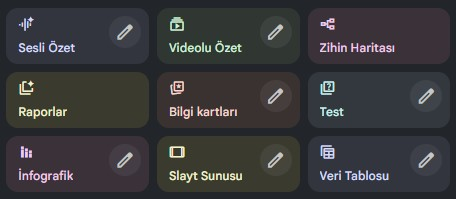
\includegraphics[width=\textwidth, height=1\textheight, keepaspectratio]{figures/notebooklm.jpg}
        \end{column}
    \end{columns}
\end{frame}
